\section{Deoxyribonucleic acid (DNA)}

\begin{wrapfigure}{r}{0.23\textwidth}
  \begin{center}
    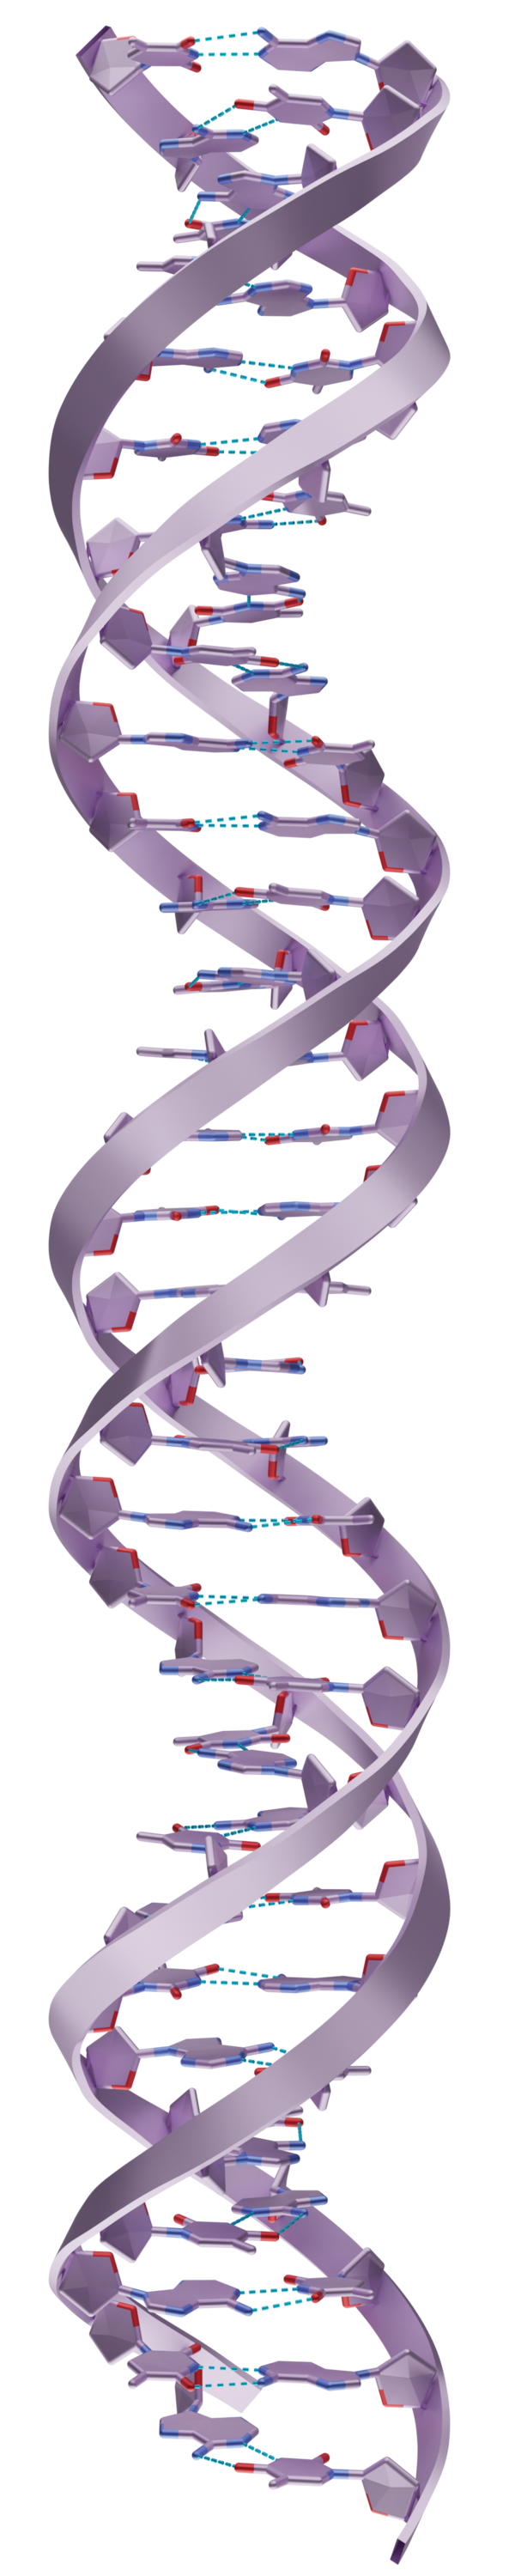
\includegraphics[width=0.20\textwidth]{Figures/DNAStrand.png}
  \end{center}
  \caption{caption nog maken}
\end{wrapfigure}

Deoxyribonucleic acid (DNA) is a long biopolymer composed of two strands, commonly found
in its characteristic double helix structure. DNA is most famously know for storing the
genetic code of organisms in the nucleus of their cells. The existence of this genetic
code was already
postulated by the Greek philosopher Aristotle. He developed a heredity theory, based
upon "blueprints", in which he tried to explain why physical traits where passed on from
generation to generation. This theory would go unnoticed until in 1869
Friedrich Meicher discovered a new microscopic substance found on discarded
surgical bandages. He would call this substance "Nuclein" since it originated
form the nucleus of the cell. Later it was found that this new substance, currently known
as "Deoxyribonucleic acid" or DNA, plays an important role as a blueprint for the
perpatuation of living matter.

The structure of DNA was first determined by Rosalind Franklin using X-ray
crystallography. Later this research was published by Watson and Crick [.], who concluded
that DNA consists of two individual strands, coiled around each other in a double helical
structure. Each strand is a chain of monomers, which we call nucleotides. A nucleotide is
made up of a
deoxyribose sugar, phosphate group and one of four nitrogenous bases: cytosine(C),
guanine(G), adenine(A) or thymine(T). The covalent bonds that give both strands structure
are formed between consecutive phosphate groups, which together make up the DNA backbone.
To form the double helix, two backbones are held together by
selective hydrogen bonds occurring between corresponding bases of opposing strands. These
dipole interactions give rise to a selection rule, forming only A-T and C-G base pairs.

Since the binding of the two strands is mediated by hydrogen bonding, association and
dissociation is possible. The study of these processes is called DNA thermodynamics. The
dissociation process of double stranded DNA (dsDNA) is called DNA melting, resulting in
two individual strands of single stranded DNA (ssDNA). The reverse process is called DNA
hybridisation, which is the selective binding of complementary nucleotides to form dsDNA.

The double helix structure of DNA comes in three different types, B-DNA, A-DNA and Z-DNA,
all having a slightly different geometric arrangement. In nature the B-form is most
commonly observed, which is characterised by a right-handed helix and the coplanarity
between the complementary bases as shown in Fig. ... . A helical twist of B-DNA consists
of around 10 base pairs, having a net helical pitch of $0.34 nm$. During this thesis,
when analysing DNA we refer to the B-DNA form.

When studying DNA the statistical theory of polymer physics is a useful tool. An
atomistic resolution is not always needed to accurately describe processes involving
relatively long DNA strands.  Reducing the complexity of DNA to the monomer level is
often justified, allowing us to use more general results in polymer physics.


